\noindent
\begin{tabular}{cc}
\begin{minipage}[b]{0.60\textwidth}
\begin{exerciseS}[Efflusso da serbatoio]
Si consideri il serbatoio rappresentato in figura, $D=2\ m$, 
$H=4.4\ m$ al cui interno \`{e} contenuta acqua, 
$\overline{\rho}=999\,{kg/m^3}$. 
Supponendo il fluido non viscoso, determinare la velocit\`{a} di 
efflusso del fluido dall'ugello del serbatoio, $h=0.4\ m$ 
e $d = 1\ cm$, e la sua portata, sia in massa sia in volume.

($U = 8.86\ m/s$, $Q=6.96\, 10^{-4}\ m^3/s$, $\overline{Q}=0.695\ kg/s$)
\end{exerciseS}
\end{minipage}
&
\begin{minipage}{0.35\textwidth}
   \begin{center}
   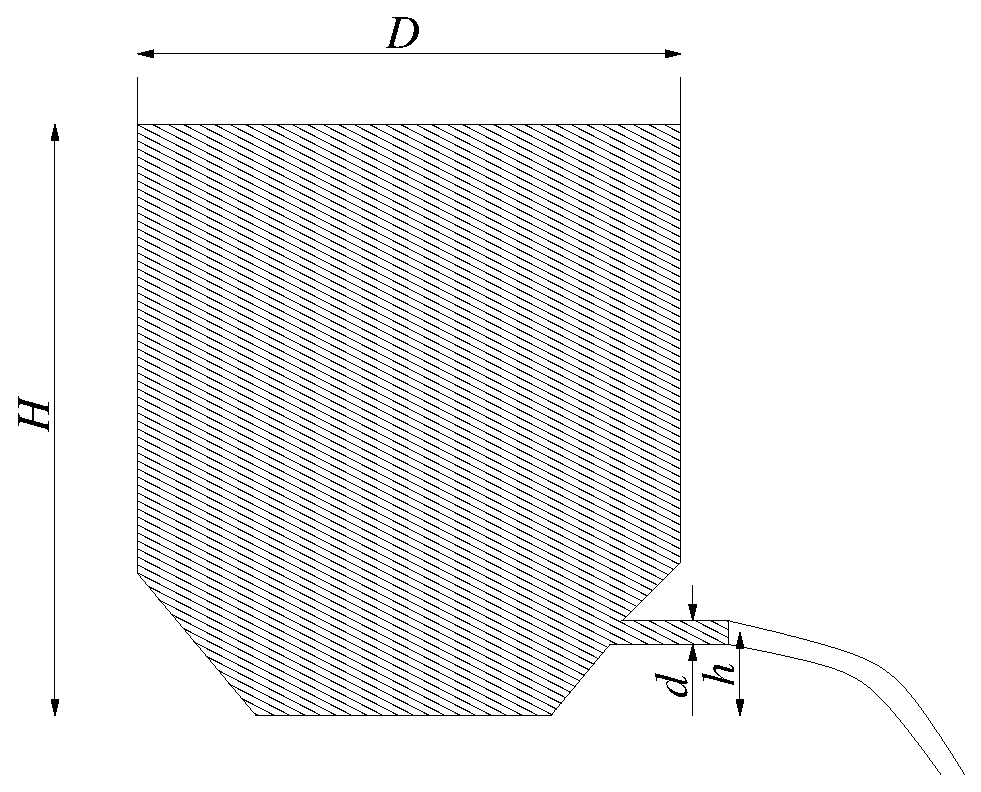
\includegraphics[width=0.90\textwidth]{./fig/serbatoio.eps}
   \end{center}
\end{minipage}
\end{tabular}

\sol

\partone
 Teorema di Bernoulli, nel caso incomprimibile, non viscoso, "stazionario" (da come è
 fatto il disegno, il livello del serbatorio sembra diminuire...assumiamo che così non sia), con forze che ammettono
potenziale e dominio semplicemente connesso.
Se si fa l'ipotesi che il flusso sia irrotazionale sulla sezione di ingresso, nel caso non viscoso, 
si mantiene irrotazionale ovunque (equazione della vorticità).
\begin{equation}
  \frac{D \bm{\omega}}{Dt} = (\bm{\omega} \cdot \bm{\nabla}) \bm{u}
\end{equation}

Si può quindi scrivere il teorema di Bernoulli nella forma:
\begin{equation}
  \frac{P}{\rho} + \frac{|\bm{u}|^2}{2} + gh = \text{cost}
\end{equation}

\parttwo
 Il problema si risolve mettendo a sistema il teorema di Bernoulli (opportunamente
semplificato; vedi sopra) con il bilancio integrale di massa. Si ipotizza che sulle due sezioni agisca la stessa pressione esterna.

\begin{equation}
\begin{cases}
  A_1 u_1 = A_2 u_2 & (massa) \\
  \frac{u_1^2}{2} + g h_1 = \frac{u_2^2}{2} + g h_2 & (Bernoulli)
\end{cases}
\end{equation}

Svolgendo i passaggi, ricordando che le superfici sono circolari, risulta:
\begin{equation}
  u_2 = \sqrt{\frac{2 g (h_1-h_2)}{1-\displaystyle\left(\frac{d_2}{d_1}\right)^4}}
\end{equation}

Si calcolano poi le portate volumetriche e di massa.
\begin{equation}
\begin{aligned}
  & Q = A_2 u_2 \\
  & \dot{m} = \rho Q
\end{aligned}
\end{equation}
